\chapter{Results}
\cite{jon}
 
\section{Pion Spectra}
\label{sec:pionSpectra}
The efficiency correction is applied track-by-track, where the efficiency of the i-th track $\epsilon_i$ is retrieved from the database, from the parameters discussed in Section~\ref{sec:efficiency}. The correction factor $C_i$ is defined as,

\begin{equation}
C_i = \epsilon_i^{-1}.
\end{equation}

Each track that is identified as a pion, is then weighted by the correction factor $C_i$, when filling any histogram. By using the track-by-track method, we can transform the track into any observable of interest, notably we can transform the  track from the lab frame into the center-of-mass (CM) frame. Before performing the transformation to the CM system recall the beam is at a small, but non-negligible, angle in the Lab frame, see Section~\ref{sec:beamangle}. The beam angle for each even is measured and a rotation is applied to all the tracks in an event, to align the beam angle along the z-axis. Doing so makes the transformation into the CM system much simpler to describe. If the beam direction is defined by a unit vector $\hat{b}$, we can define the rotation that rotates the beam into the z-axis as a rotation about an arbitrary vector $\hat{v} = \hat{b}\times\hat{z}$ where the angle between the two is given by $\cos \theta = \hat{b}\cdot\hat{z}$. 

Once all the events have been rotated to align with the z-axis, transforming from the Lab to the CM frame is done by a Lorentz transformation. Where the 4-momentum vector in the lab frame is defined as $\textbf{P} = (E/c,p_x,p_y,p_z)$. Where the corresponding Lorentz transform into the CM frame along the beam (z-axis) is defined as,

\begin{equation}
A = \begin{pmatrix}
1 & 0 & 0 & 0\\
0 & 1 & 0 & 0\\
0 & 0 & \gamma & -\beta \gamma\\
0 & 0 & -\beta \gamma & \gamma
\end{pmatrix},
\end{equation}

where $\beta$, describes the velocity of the CM system, and $\gamma=\sqrt{1-\beta^2}^{-1}$. The parameter $\beta$ can be determined from the total momentum of the system in the Laboratory frame $P = \sqrt{ T_{P}^2 - M_{T}^2}$ and the total energy of the system $E = T_{P} + M_{P} + M_{T}$ as $\beta = -P/E$, where the (-) sign denotes the correct direction for transforming from the Lab to the CM frame. The CM transformed track is defined as $p^{CM} = \textbf{A}p^{Lab}$.


%need to add error analysis
%systematic error analysis


Figure~\ref{fig:pionspectra} shows the pion CM kinetic energy spectra for both the $\tin{132}{124}$ and $\tin{108}{112}$ systems. This data marks the first pion spectral data at sub-threshold energies, extending to very low pion energies. The coulomb potential works to accelerate $\pi^+$ and decelerate $\pi^-$ particles due to the positive charge of the nuclear medium. The coulomb barrier prevents the production of low energy $\pi^+$, which is why there is a reduction in the phase space around zero kinetic energy. 

\begin{figure}[!htb]
\centering
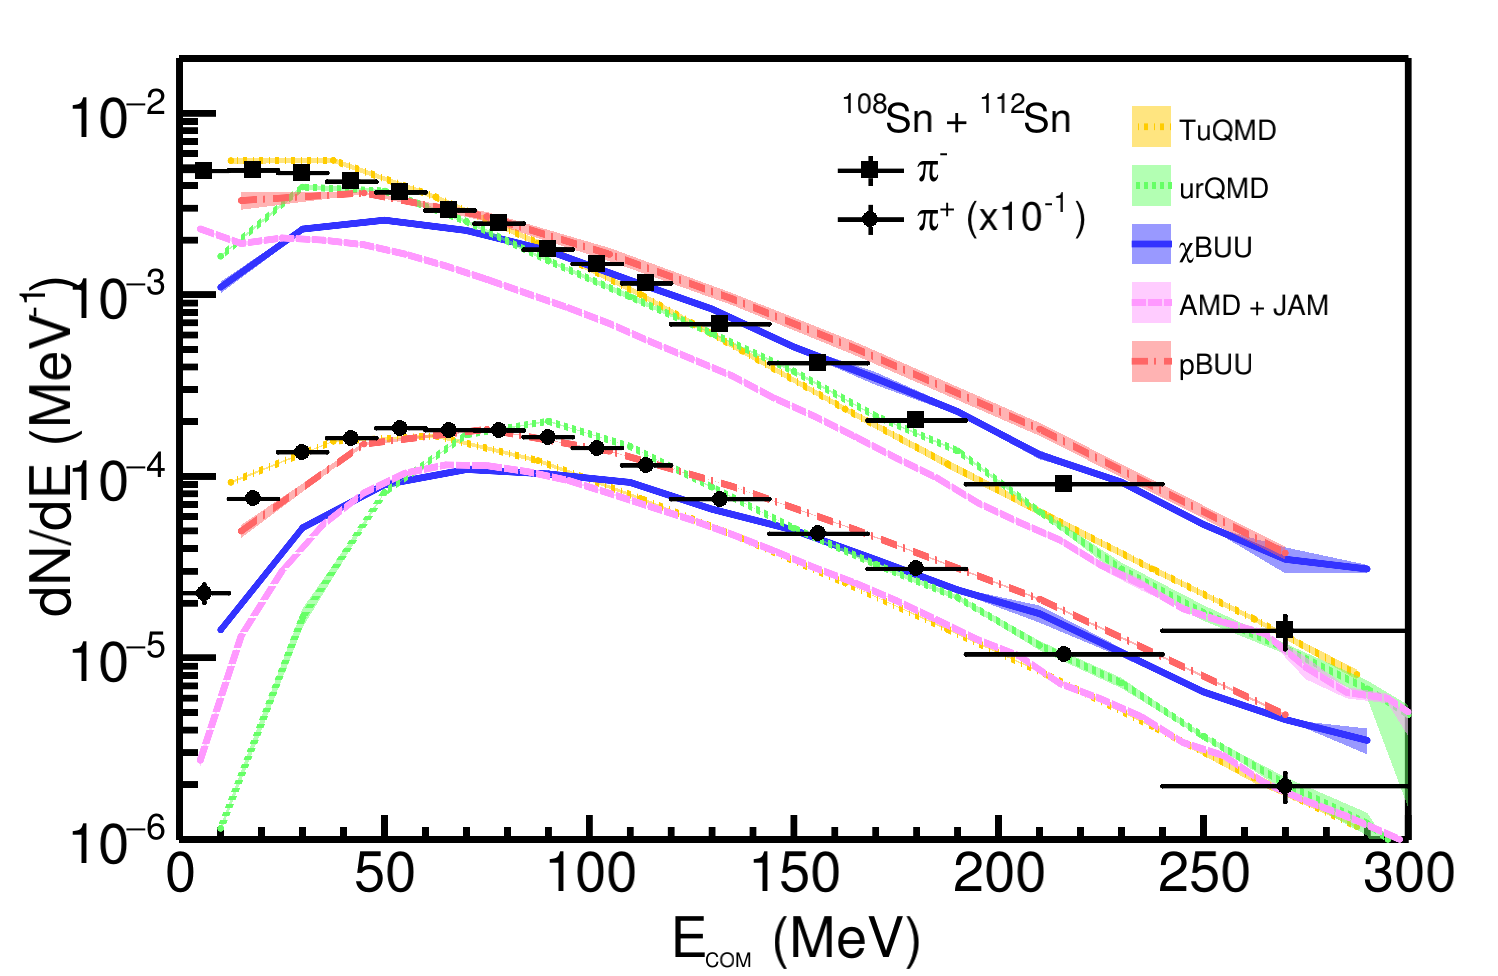
\includegraphics[width=\textwidth]{pionSpectra.png}
\caption{Pion spectra. }
\label{fig:pionspectra}
\end{figure}


%Add figure on Glauber model 
%Add figure on comparison to FOPI data

\section{Pion Yield}

The integrated pion yield for both systems and the $\pi^-/\pi^+$ ratio is listed in Table~\ref{tb:pionyield}, where the systematic errors are the first error bar and the statistical error is listed next. It is remarkable that the pion ratio is significantly greater than the N/Z of the system which is what is expected in the Delta Resonance model or under the assumption of chemical equilibrium which is $\pi^-/\pi^+ = (N/Z)^2$ CITE HERE; 2x in the $\tin{132}{124}$ system and 1.4x in the $\tin{108}{112}$ system. The pion ratio was hypothesized to be proportional to the high density N/Z ratio of the early system, where the other effects such as pion absorption and re-emission would dilute the effect and lower the ratio as the system tends toward isospin equilibrium. A na\"ive interpretation would be the high density N/Z fraction is much higher for some reason than the two systems, though, the system spends very little time in this state which would require a very soft Symmetry Energy. A more likely conclusion is the mechanisms involved in pion productions via the $\Delta(1232)$ resonance is more complicated than the simple $(N/Z)^2$ relation. For example the $\Delta$ resonance potential has an iso-scalar component (independent of iso-spin) and an iso-vector component. The nature of these two potentials is still unknown CITE HERE, and the role it plays in pion production has shown to be very important CITE HERE.


\begin{table*}\centering
\ra{1.3}
\begin{tabular}{@{}cccc@{}}\toprule
System & $\pi^-$ & $\pi^+$ & $Y(\pi^-)/Y(\pi^+)$  \\
\midrule
$\tin{132}{124}$ & 0.717(24)(4) & 0.148(5)(2) & 4.84(10)(6)  \\
$\tin{108}{112}$ & 0.399(14)(3) & 0.200(8)(2) & 1.99(4)(3)  \\
%$\tin{132}{124}$ & \numerr{0.717}{0.024}{0.004} & \numerr{0.148}{0.005}{0.002} & \numerr{4.84}{0.10}{0.06}  \\
%$\tin{108}{112}$ & \numerr{0.399}{0.014}{0.003} & \numerr{0.200}{0.008}{0.002} & \numerr{1.99}{0.04}{0.03}  \\
\bottomrule
\end{tabular}
\caption{Total pion yield.}
\label{tb:pionyield}
\end{table*}


We have compared the total pion yields and ratios to the 6 common transport codes for the systems measured. The table of the transport codes are listed in Appendix~\ref{tb:pionyieldTheory}. Figure~\ref{fig:totalpiYield} shows the total pion yield for the four systems measured as compared with the codes. The codes plotted here are only the soft symmetry energy since the variation in code is much larger than the intra-code variation between different Symmetry Energies. While some codes make a reasonable approximation of a particular charge pion, no code reasonably predict both. 

\begin{figure}[!htb]
\centering
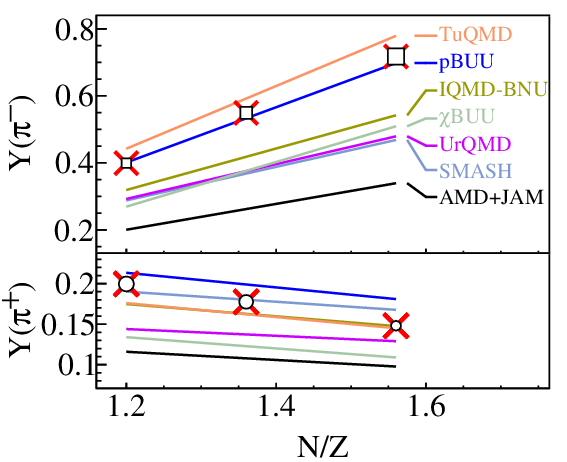
\includegraphics[width=.8\textwidth]{totalpiYield.png}
\caption{Total pion yields as compared with 6 common transport codes.}
\label{fig:totalpiYield}
\end{figure}

Figure~\ref{fig:totalpiRatio} shows the total single pion ratio and the double ratio of the $\tin{132}{124}$ and $\tin{108}{112}$ system. Here, the variation between codes is much larger than the variation between the Symmetry Energy within a particular code. The Symmetry Energy variation of two codes -- $\chi$BUU and TuQMD -- is plotted as a wide band in the single ratio and all codes in the double ratio; the data band represents the data error bar. Certainly the variation between Symmetry Energy in the $\tin{132}{124}$, though small, still exists in many of the codes as predicted initially CITE HERE BAO ANN. The small error bars in the data also would allow for a detailed analysis to extract a constraint of the Symmetry Energy, if the variation between codes could be solved. 



\begin{figure}[!htb]
\centering
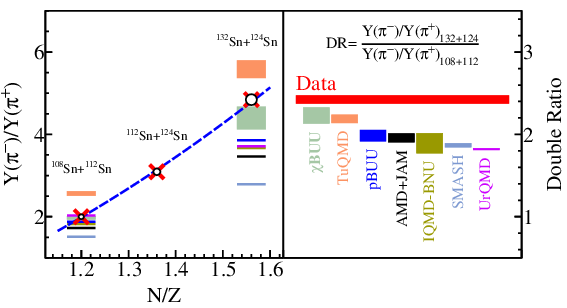
\includegraphics[width=\textwidth]{totalpiRatio.png}
\caption{Total pion ratio and double ratio compared with 6 common transport codes.}
\label{fig:totalpiRatio}
\end{figure}



\section{Pion Spectral Ratio}


\begin{figure}[!htb]
\centering
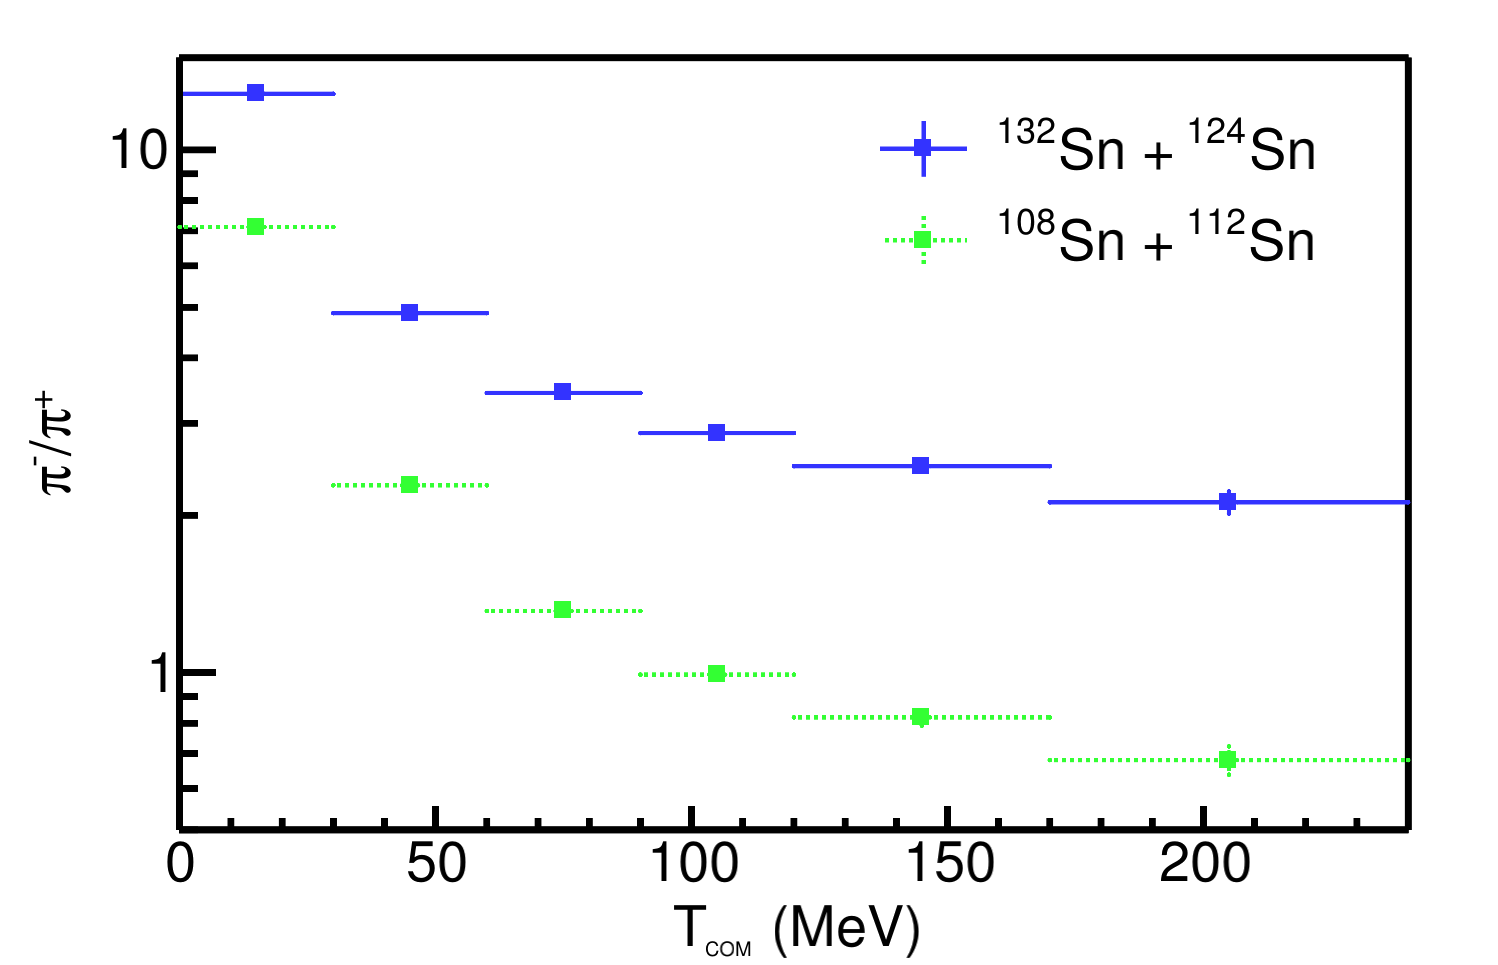
\includegraphics[width=\textwidth]{singleRatio.png}
\caption{Single ratio spectra}
\label{fig:SRspectra}
\end{figure}

The pion spectral ratio is a promising observable in particular it may be more sensitive to the high density regions of the early collision. In theory the high energy pions are more likely to exit the nuclear medium earlier, and therefore be less prone to effects such as pion absorption and re-emission which dilute the sensitivity of the pion observable to the high density behavior. Also low energy pions are more likely to be affected by other effects such as the $\Delta$ potential in medium CITE HERE BAO AN. If we integrate the total pion yield we combine these two regions of low and high energy pions. Instead we can construct the $Y(\pi^-)/Y(\pi^+)$ ratio as a function of the kinetic energy in the CM system. 

%Mention and cite appendix for systematics

Figure~\ref{fig:SRspectra} shows the pion spectral ratio for both systems, which was measured with a high degree of accuracy. The general hyperbolic shape comes from the Coulomb force on the two charged pion spectra mentioned in Section~\ref{sec:pionSpectra}. Naturally the pion ratio is smaller for less neutron poor system, i.e. less neutron-neutron collisions produce less $\pi^-$. The bin size of the last bin was increased to reduce the statistical error bars since the number of pions, especially the $\pi^+$, is reaching the limits of the measured distribution. 



%Add figure of Theory for pion ratios

\section{Pion Double Ratio}
%Add figure of Theory for pion ratios

\begin{figure}[!htb]
\centering
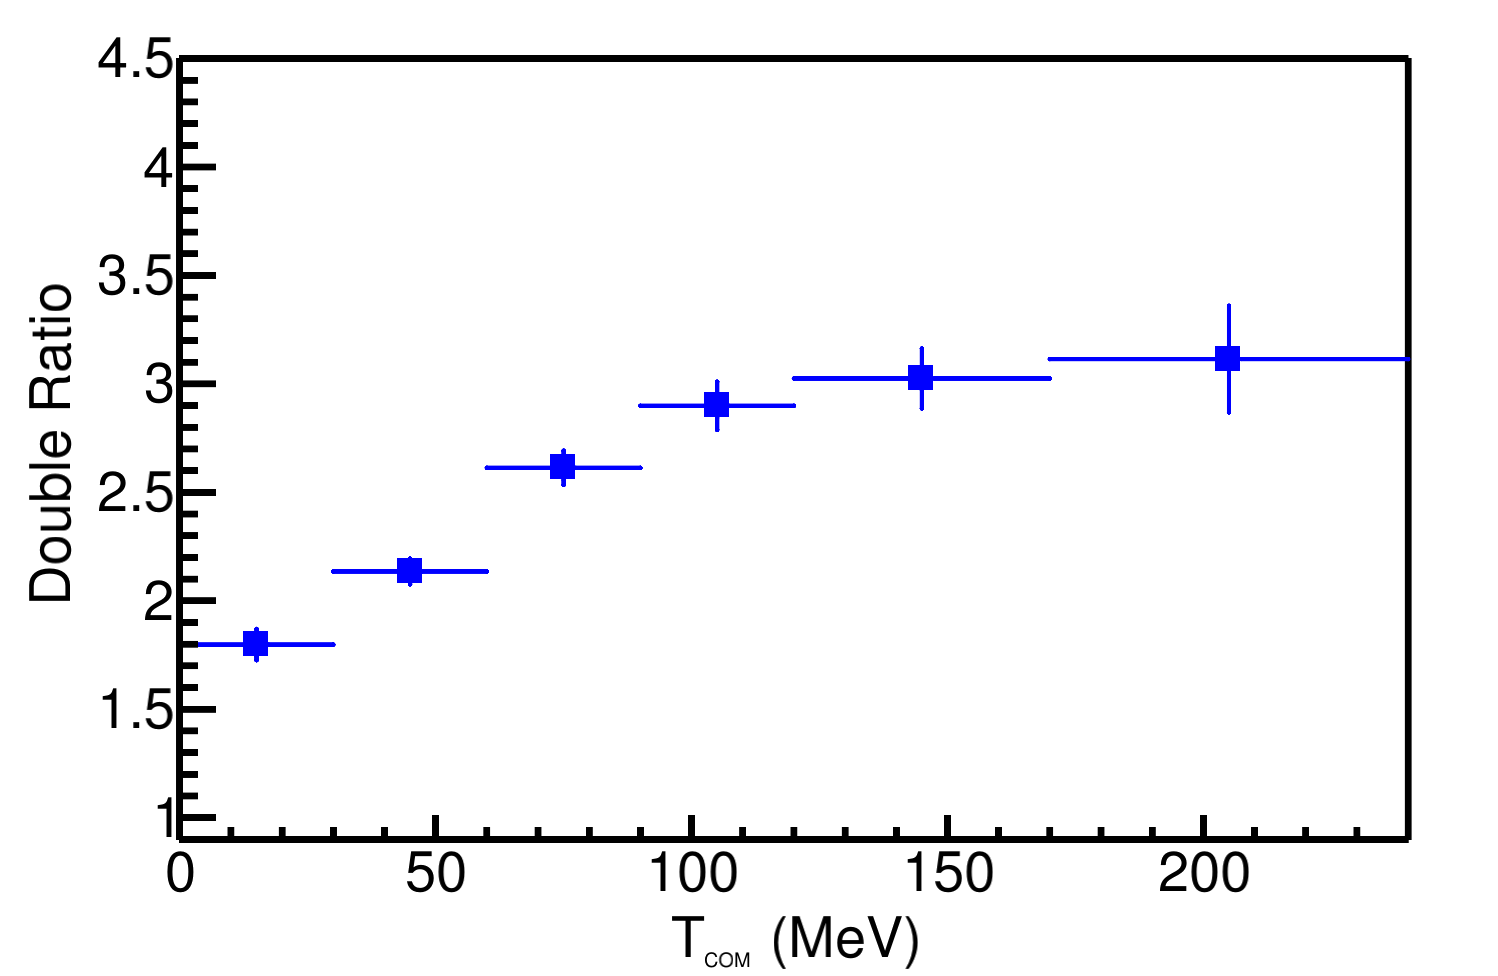
\includegraphics[width=\textwidth]{doubleRatio.png}
\caption{}
\label{fig:spectraDR}
\end{figure}

Another promising observable is the spectral double ratio. In a similar way described in Section~\ref{sec:doubleRatio} we would expect systematic uncertainties in the experiment, and even in the theory, to cancel out. For the same reasons as the pion spectral ratio, we would expect the high energy pions to be more sensitive to the high density region of the early collision. 



\section{Comparison to Previous Data Sets (FOPI)}


\begin{figure}[!htb]
\centering
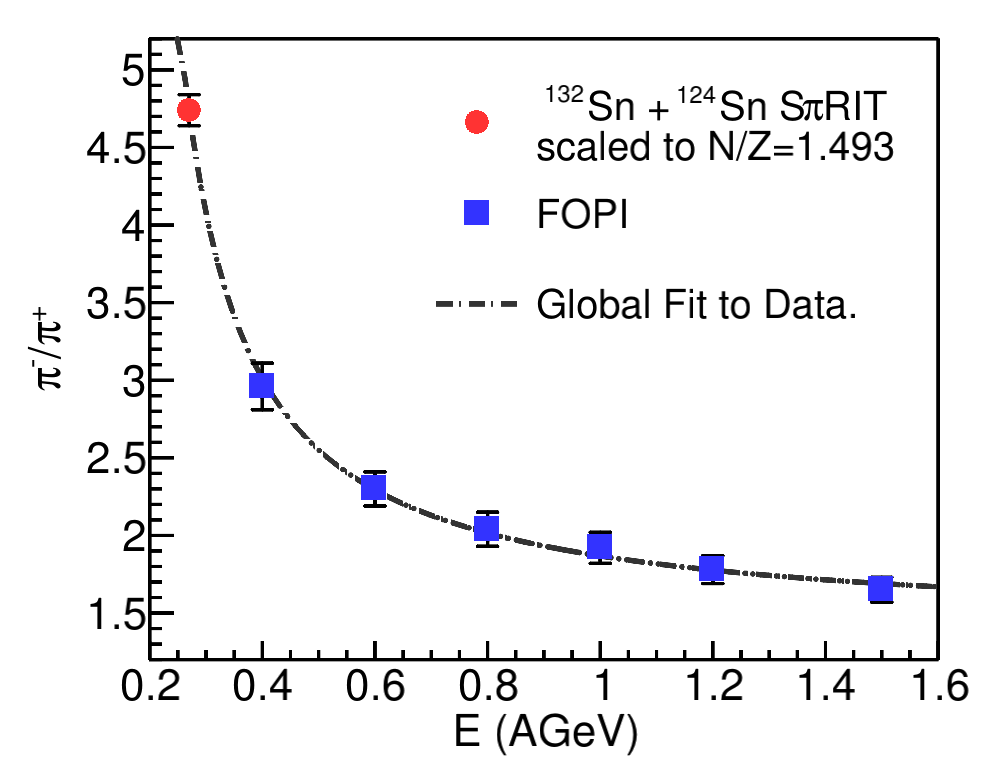
\includegraphics[scale=.4]{fopi_pionratio_comp}
\caption{Comparing the total $\pi^-/\pi^+$ ratio of the $\tin{132}{124}$ system to the ${}^{197}$Au + ${}^{197}$Au data from the FOPI collaboration. The \spirit TPC data was scaled by a factor to compare to the lower N/Z of the Au + Au system. This was extracted from measuring the N/Z dependence measured in the experiment. }
\label{fig:fopiPionRatio}
\end{figure}

The FOPI collaboration has measured the total pion multiplicity resulting from ${}^{197}Au + {}^{197}Au$ collisions at several, higher beam energies. In the $\tin{132}{124}$ data  $N/Z=1.56$ where as in the ${}^{197}Au + {}^{197}Au$, $N/Z=1.493$. The pion ratio is proportional to the $N/Z$ of the system. Since 4 beams were measured in this experiment, the $N/Z$ dependence was measured as seen in Fig.~\ref{fig:totalpiRatio}. Here the dependence is fitted with a 2-nd order polynomial fit. The pion ratio in the $\tin{132}{124}$ data  was scaled by the ratio between $N/Z=1.56$ and 1.493. Figure~\ref{fig:fopiPionRatio} shows the scaled pion ratio as compared with the FOPI pion ratio from literature CITE HERE. The fitted function has the functional form of $p_1(E - p_2)^{-2}$ where $p_1$ and $p_2$ are free parameters, and is meant to guide the eye. It is worth mentioning that the pion ratio observed in the FOPI \SI{400}{\MeVA} setting was already considerably higher than what is expected from the $(N/Z)^2$ delta resonance model CITE HERE. Scaling the other systems in the \spirit TPC data leads to almost the exact same value of $\mathrm{Y}(\pi^-)/\mathrm{Y}(\pi^+) = \num{4.82}$.



\section{Comparison to Theory}
%Add figure of Pion spectra for different theory 
%Reference paper for multiple theories

Here we will compare with 7 different commonly used transport theoretical codes. These codes took part in a large collaboration effort to compare the codes to each other. The goal of these comparison projects was to standardize the input into each code to systematically go through the details in each code comparing things such as initialization of nuclei, stability of the code, numerical handing of pauli-blocking, etc CITE HERE. These codes were taken in their best state, without any prior knowledge of the experimental data, and simulated the 4 systems measured in the \spirit TPC at an impact parameter of \SI{3}{\femto\metre} at \SI{270}{\MeVA} beam energy. Each code differs in its treatment of pion and $\Delta$ dynamics. Some codes contain modifications to the pion in nuclear matter, usually by including a pion optical potential. Some codes include the iso-scalar and the iso-vector delta potential which are not very well constrained but are important in the production of pions CITE HERE.


\section{Systematic Errors and Cut Variations}
\label{sec:cutvar}
The particular track quality cuts described in Section~\ref{sec:qualitycut} are there to reduced the contamination from poorly reconstructed tracks which contribute to the background in the PID spectra. The best set of values were found for all the data sets which include the charged particle multiplicity of the event, dOCA, and the number of clusters cut. By varying the cuts in both the data and the MC efficiency, we can evaluate the analysis to see if there are any systematic dependencies on the observable we plot. But varying the cuts undoutably means as the cut get tighter, and less data is included, the statistical error bar will increase making it difficult to compare to more loose cuts. This is mitigated by looking at the uncorrelated error described in \cite{dataAnalysis}. Here if the systematic trend of the observable is much larger than the statistical error bars on the default cuts and the uncorrelated error bars, then there is some systematic trend that either exists due to physics or some error or miscalculation in the analysis. It is usually not recommended to estimated systematic error bars using this method, but sometimes is the only way. 

Here we will discuss the particular analysis using the total pion ratio as the example. Figure~\ref{fig:totalRatioError} shows the total pion as a function of several cut variations, where one cut is varied and all the others are held constant. Three cuts are of particular interest, the event multiplicity, dOCA, and the number of cluster cut. Figure~\ref{fig:clustTotalRatio} shows the variation as the number of cluster cut is varied. The default cut used is > 20 clusters which is represented by the middle point. The red bars represent the statistical error of this default value. The error bars on the other points are the uncorrelated error bars as described by the prescription in \cite{dataAnalysis}. Here it is clear that there is a systematic bias in the pion ratio as a function 

%show the pim total yield 
%discuss others in the apendix 


\begin{figure}[!htb]
     \centering
     \begin{subfigure}[b]{\textwidth}
         \centering
         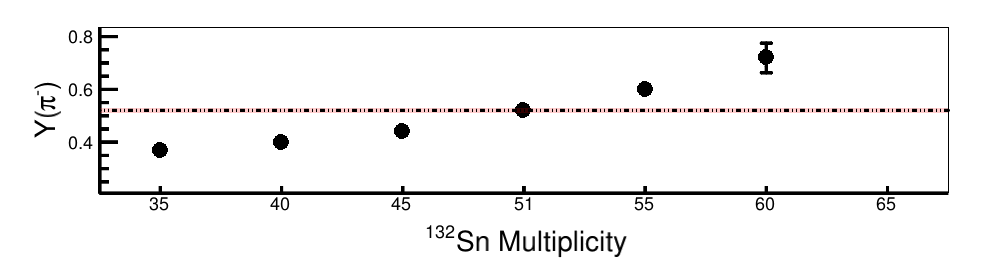
\includegraphics[width=\textwidth]{132Sn_Multiplicity_NoEC_pimTotal}
         \caption{No efficiency correction.}
         \label{fig:multCutVar}
     \end{subfigure}
     \hfill
    \begin{subfigure}[b]{\textwidth}
         \centering
         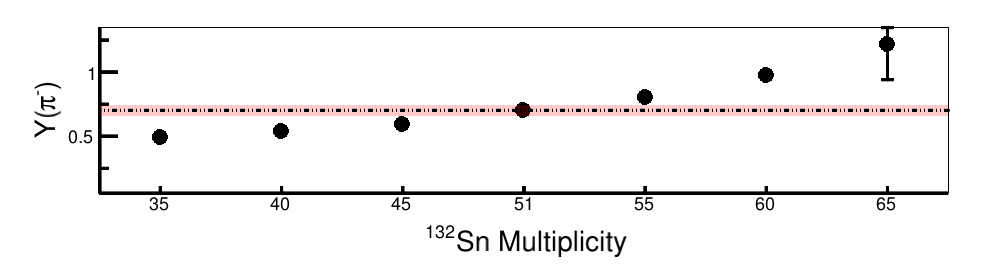
\includegraphics[width=\textwidth]{132Sn_Multiplicity_pimTotal}
         \caption{Efficiency corrected.}
         \label{fig:multCutVar}
     \end{subfigure}
     \hfill
\caption{Y($\pi^-$) when varying the ${}^{132}$Sn charged particle multiplicity cut. }
\label{fig:cutVar}
\end{figure}



\begin{figure}[!htb]
     \centering
     \begin{subfigure}[b]{\textwidth}
         \centering
         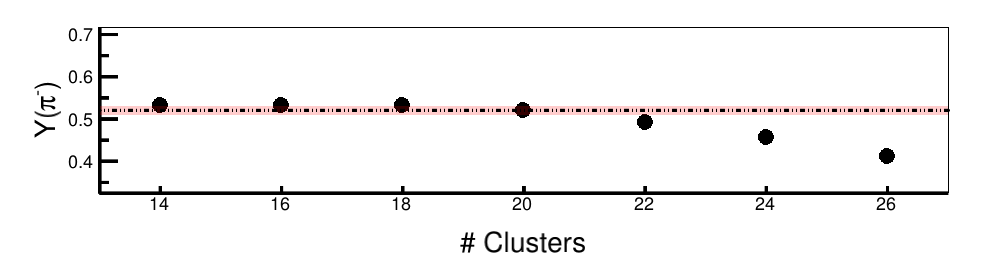
\includegraphics[width=\textwidth]{Clusters_NoEC_pimTotal}
         \caption{Before efficiency correction.}
         \label{fig:pim_clustVar_NoEC}
     \end{subfigure}
     \hfill
    \begin{subfigure}[b]{\textwidth}
         \centering
         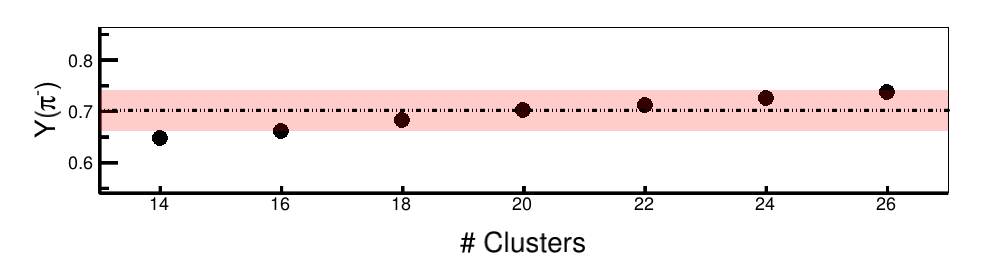
\includegraphics[width=\textwidth]{Clusters_pimTotal}
         \caption{After efficiency correction.}
         \label{fig:pim_clustVar_EC}
     \end{subfigure}
     \hfill
\caption{Y($\pi^-$) when varying the number of cluster cut of the tracks.}
\label{fig:pim_clustVar}
\end{figure}




\begin{figure}[!htb]
     \centering
     \begin{subfigure}[b]{\textwidth}
         \centering
         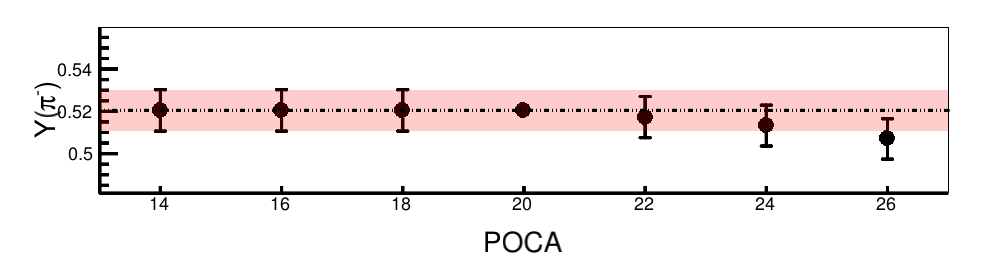
\includegraphics[width=\textwidth]{POCA_NoEC_pimTotal}
         \caption{No efficiency correction.}
         \label{fig:pim_cutVarPOCA_NoEC}
     \end{subfigure}
     \hfill
    \begin{subfigure}[b]{\textwidth}
         \centering
         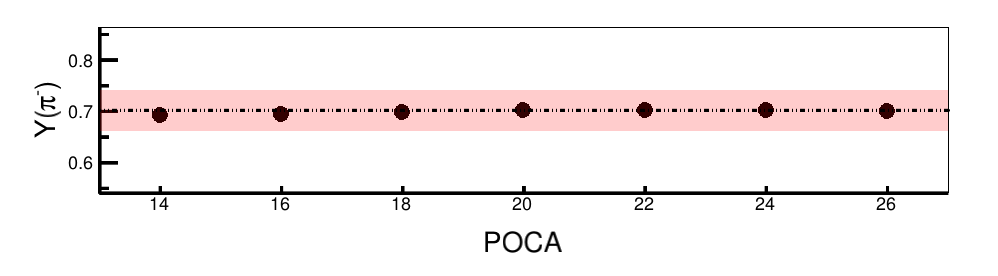
\includegraphics[width=\textwidth]{POCA_pimTotal}
         \caption{Efficiency corrected.}
         \label{fig:pim_cutVarPOCA_EC}
     \end{subfigure}
     \hfill
\caption{Y($\pi^-$) when varying the dOCA cut.}
\label{fig:pim_cutVarPOCA}
\end{figure}
